\chapter{Results}
\label{ch:results}

All numbers are test macro-F1 unless stated otherwise. Artifacts are in
\texttt{reports/} of the code repository.

\section{Clip-level results}
\label{sec:res-clip}

On the canonical clip-level split, frozen Whisper-small embeddings with an MLP
head reach a macro-F1 of \fscore{0.917} (accuracy 0.916, $n = 1{,}329$), and
end-to-end fine-tuned XLS-R-300M reaches \fscore{0.952}, 3.5 points higher.
The MFCC baseline reaches \fscore{0.727}. \Cref{tab:clip-perclass} and
\cref{fig:perclass-clip} give the per-class scores.

\begin{table}[ht]
  \centering
  \caption{Per-class test F1, clip-level split (upper bound).}
  \label{tab:clip-perclass}
  \begin{tabular}{lccc}
    \toprule
    Class & MFCC + MLP & Frozen Whisper + MLP & Fine-tuned XLS-R \\
    \midrule
    Khulna     & 0.879 & 0.986 & 0.986 \\
    Sylhet     & 0.873 & 0.951 & 0.982 \\
    Rajshahi   & 0.781 & 0.947 & 0.980 \\
    Formal     & 0.770 & 0.970 & 0.973 \\
    Dhaka      & 0.655 & 0.913 & 0.972 \\
    Barishal   & 0.653 & 0.871 & 0.927 \\
    Chattogram & 0.597 & 0.880 & 0.924 \\
    Mymensingh & 0.651 & 0.890 & 0.912 \\
    Noakhali   & 0.688 & 0.848 & 0.910 \\
    \midrule
    Macro      & \textbf{0.727} & \textbf{0.917} & \textbf{0.952} \\
    \bottomrule
  \end{tabular}
\end{table}

\begin{figure}[ht]
  \centering
  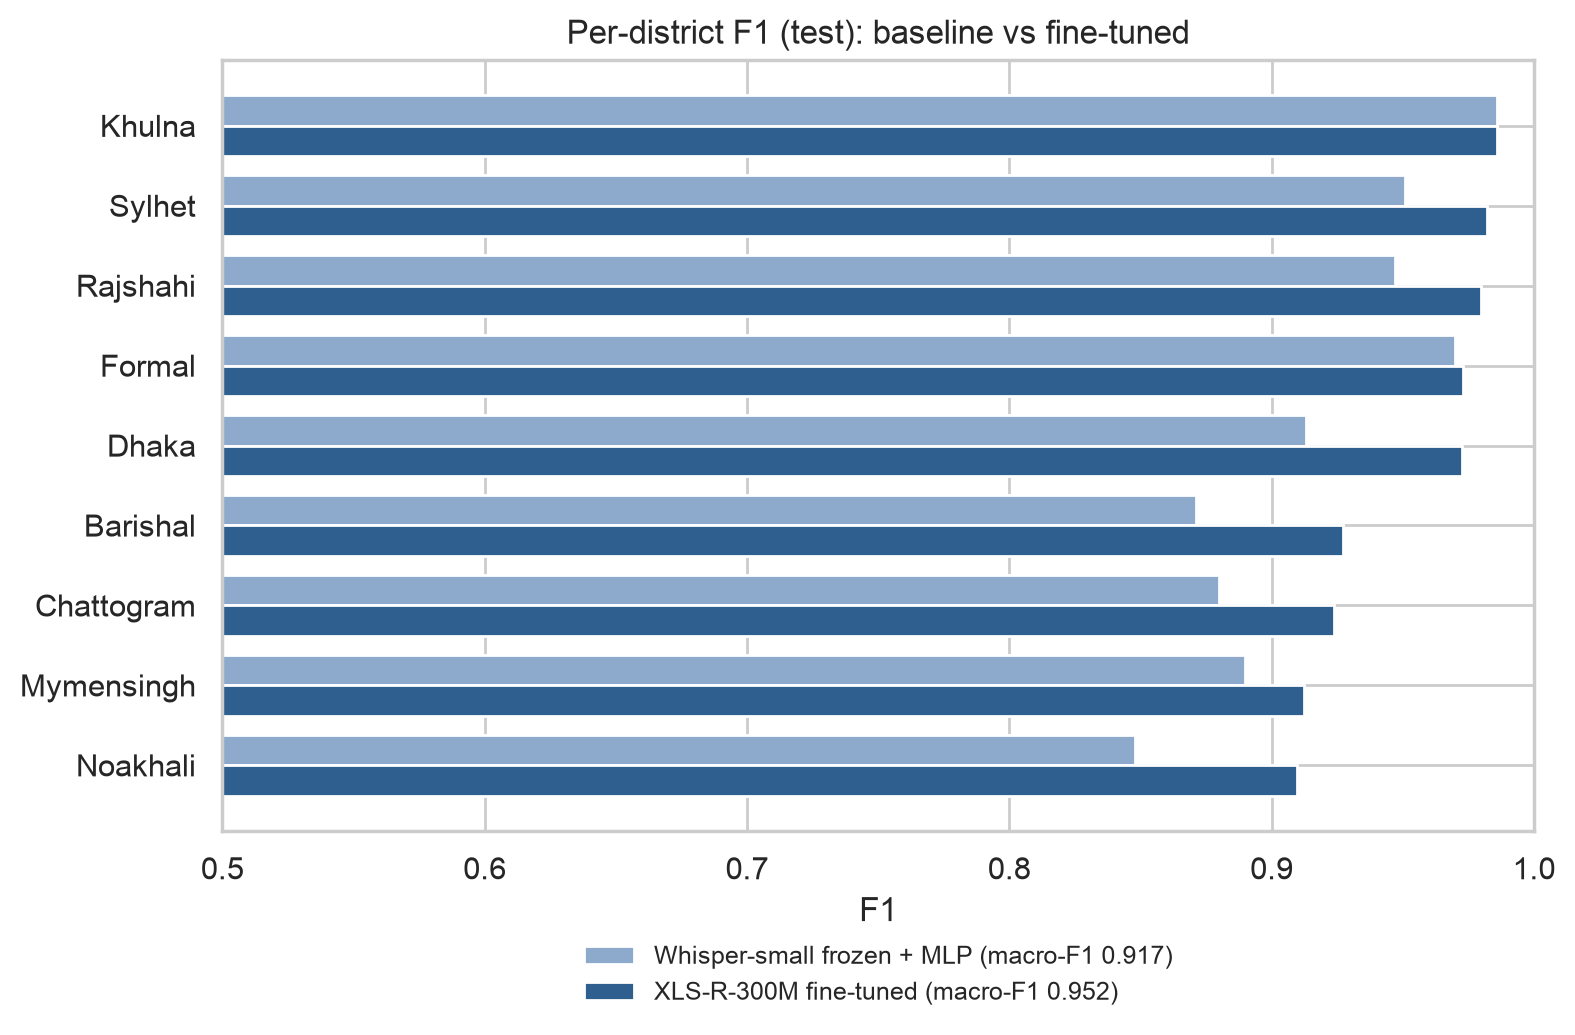
\includegraphics[width=0.85\textwidth]{per_class_f1_comparison.png}
  \caption{Per-class test F1 on the clip-level split: frozen Whisper-small with
  an MLP head against fine-tuned XLS-R-300M.}
  \label{fig:perclass-clip}
\end{figure}

Three observations follow.
\begin{itemize}
  \item Fine-tuning's gains concentrate on the frozen baseline's weakest classes:
        Noakhali (+6.1 points), Dhaka (+5.9), Barishal (+5.6) and Chattogram
        (+4.4). Task adaptation moves capacity towards the hard, acoustically
        close dialects.
  \item The dominant confusion is between Barishal and Noakhali, two southern
        coastal dialects (\cref{fig:confusion}). Fine-tuning halves it, from 31
        to 15 test errors, but does not remove it. Mymensingh, a transitional
        dialect zone, spreads its errors across its neighbours. Errors follow
        dialect geography rather than falling at random.
  \item Training converges: the 8-epoch pilot reached 0.865 and was still
        rising, while the 20-epoch run's validation score plateaus at about 0.95
        from epoch 11 (\cref{fig:training-curve}).
\end{itemize}

\begin{figure}[ht]
  \centering
  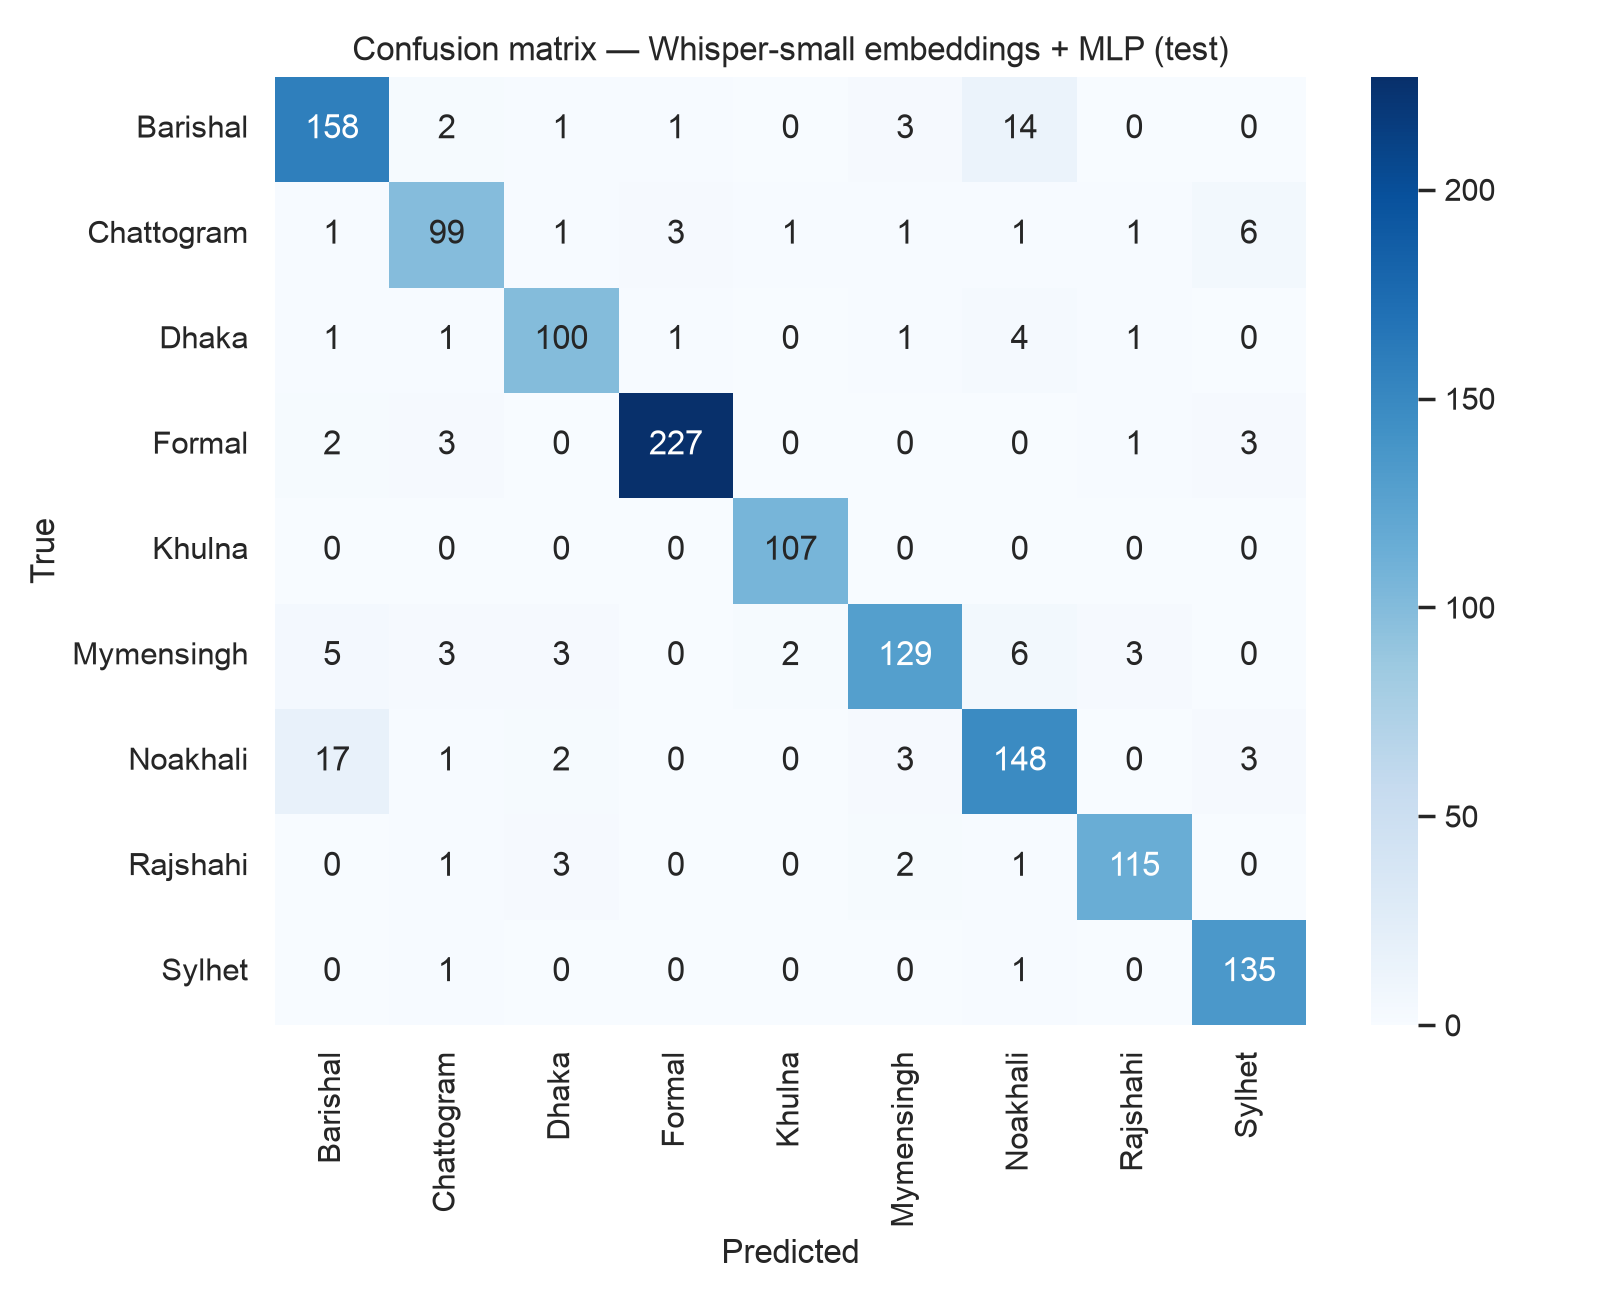
\includegraphics[width=0.64\textwidth]{confusion_matrix_baseline.png}\\[4pt]
  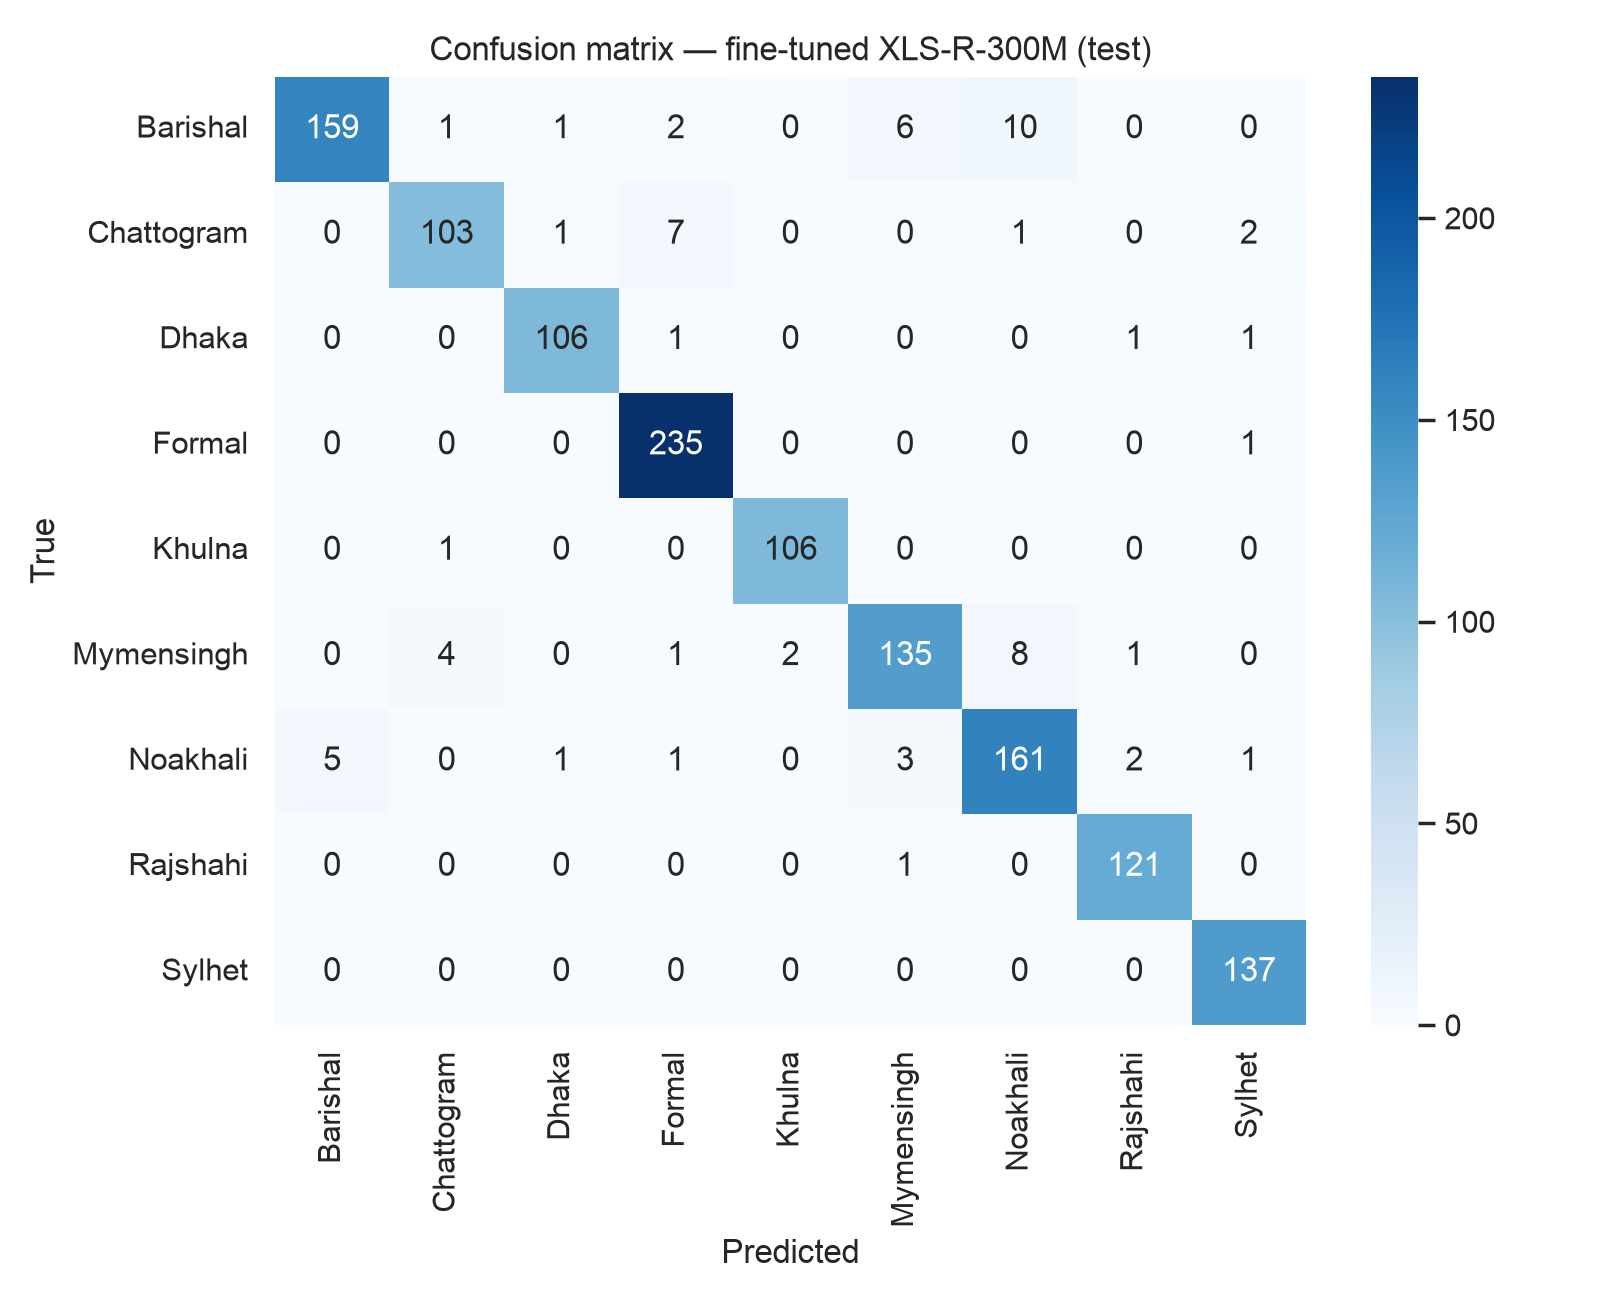
\includegraphics[width=0.64\textwidth]{confusion_matrix_xlsr.png}
  \caption{Test confusion matrices on the clip-level split. Top: frozen
  Whisper-small with an MLP head. Bottom: fine-tuned XLS-R-300M. Rows are true
  classes, columns predictions. The Barishal--Noakhali confusion falls from
  $14 + 17 = 31$ to $10 + 5 = 15$ errors.}
  \label{fig:confusion}
\end{figure}

\begin{figure}[ht]
  \centering
  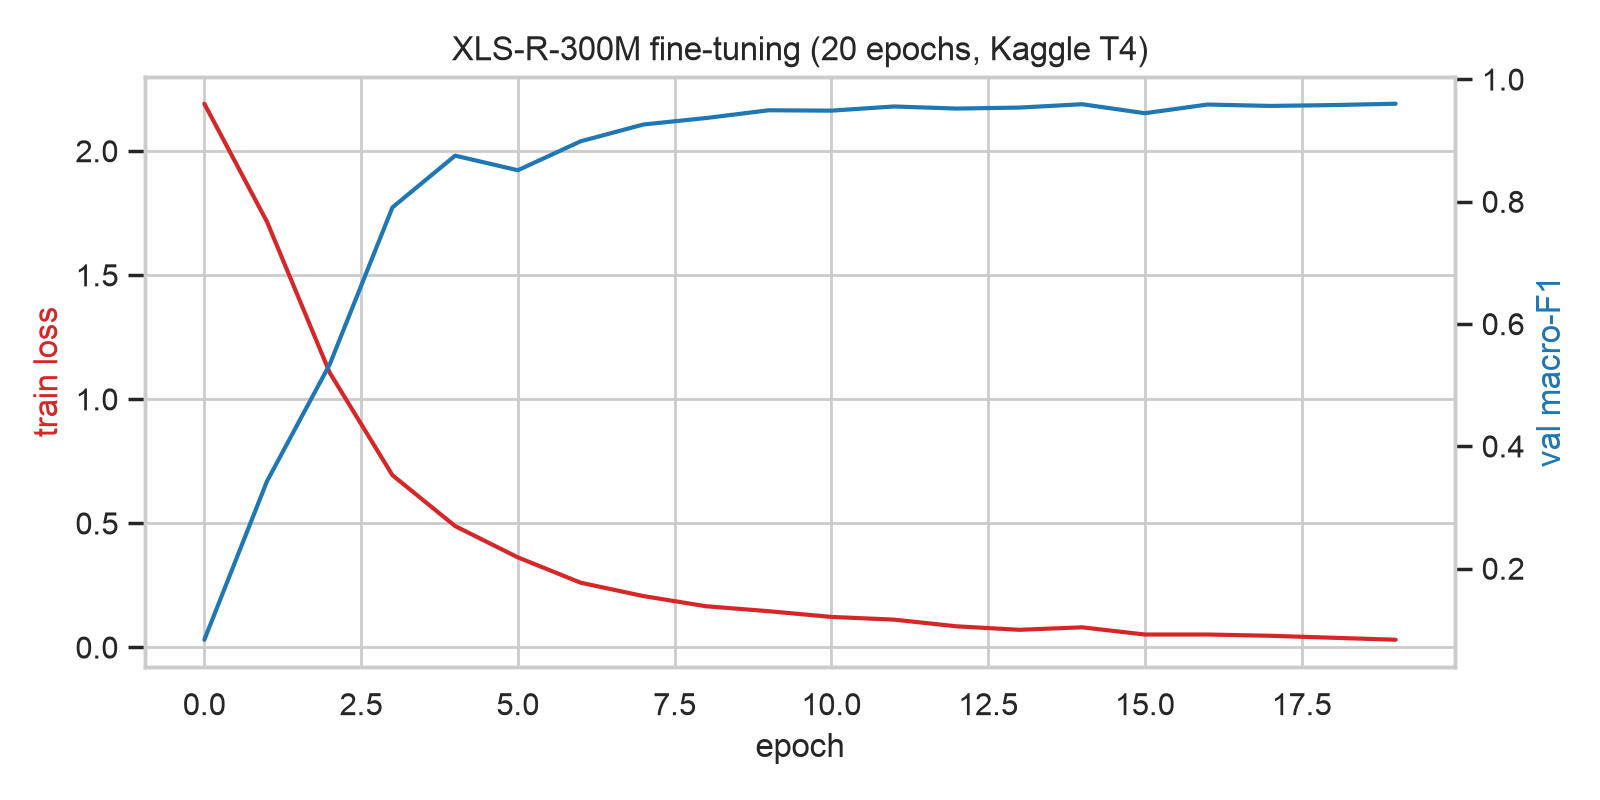
\includegraphics[width=0.85\textwidth]{training_curve_xlsr.png}
  \caption{XLS-R-300M fine-tuning on the clip-level split: training loss (red,
  left axis) and validation macro-F1 (blue, right axis) over 20 epochs on a
  Kaggle T4.}
  \label{fig:training-curve}
\end{figure}

\Cref{fig:tsne} projects frozen Whisper embeddings into two dimensions with t-SNE \citep{vandermaaten2008tsne}. Formal, Sylhet, Rajshahi and
Khulna form recognisable regions even before any task-specific training, while
Barishal, Noakhali and Mymensingh overlap heavily---the same classes the
classifiers confuse. Several small, tight clusters, such as a short arc of
Barishal clips and an isolated group of Formal clips, are the kind of
single-recording groups that the strict split is designed to keep on one side
of the train/test boundary.

\begin{figure}[ht]
  \centering
  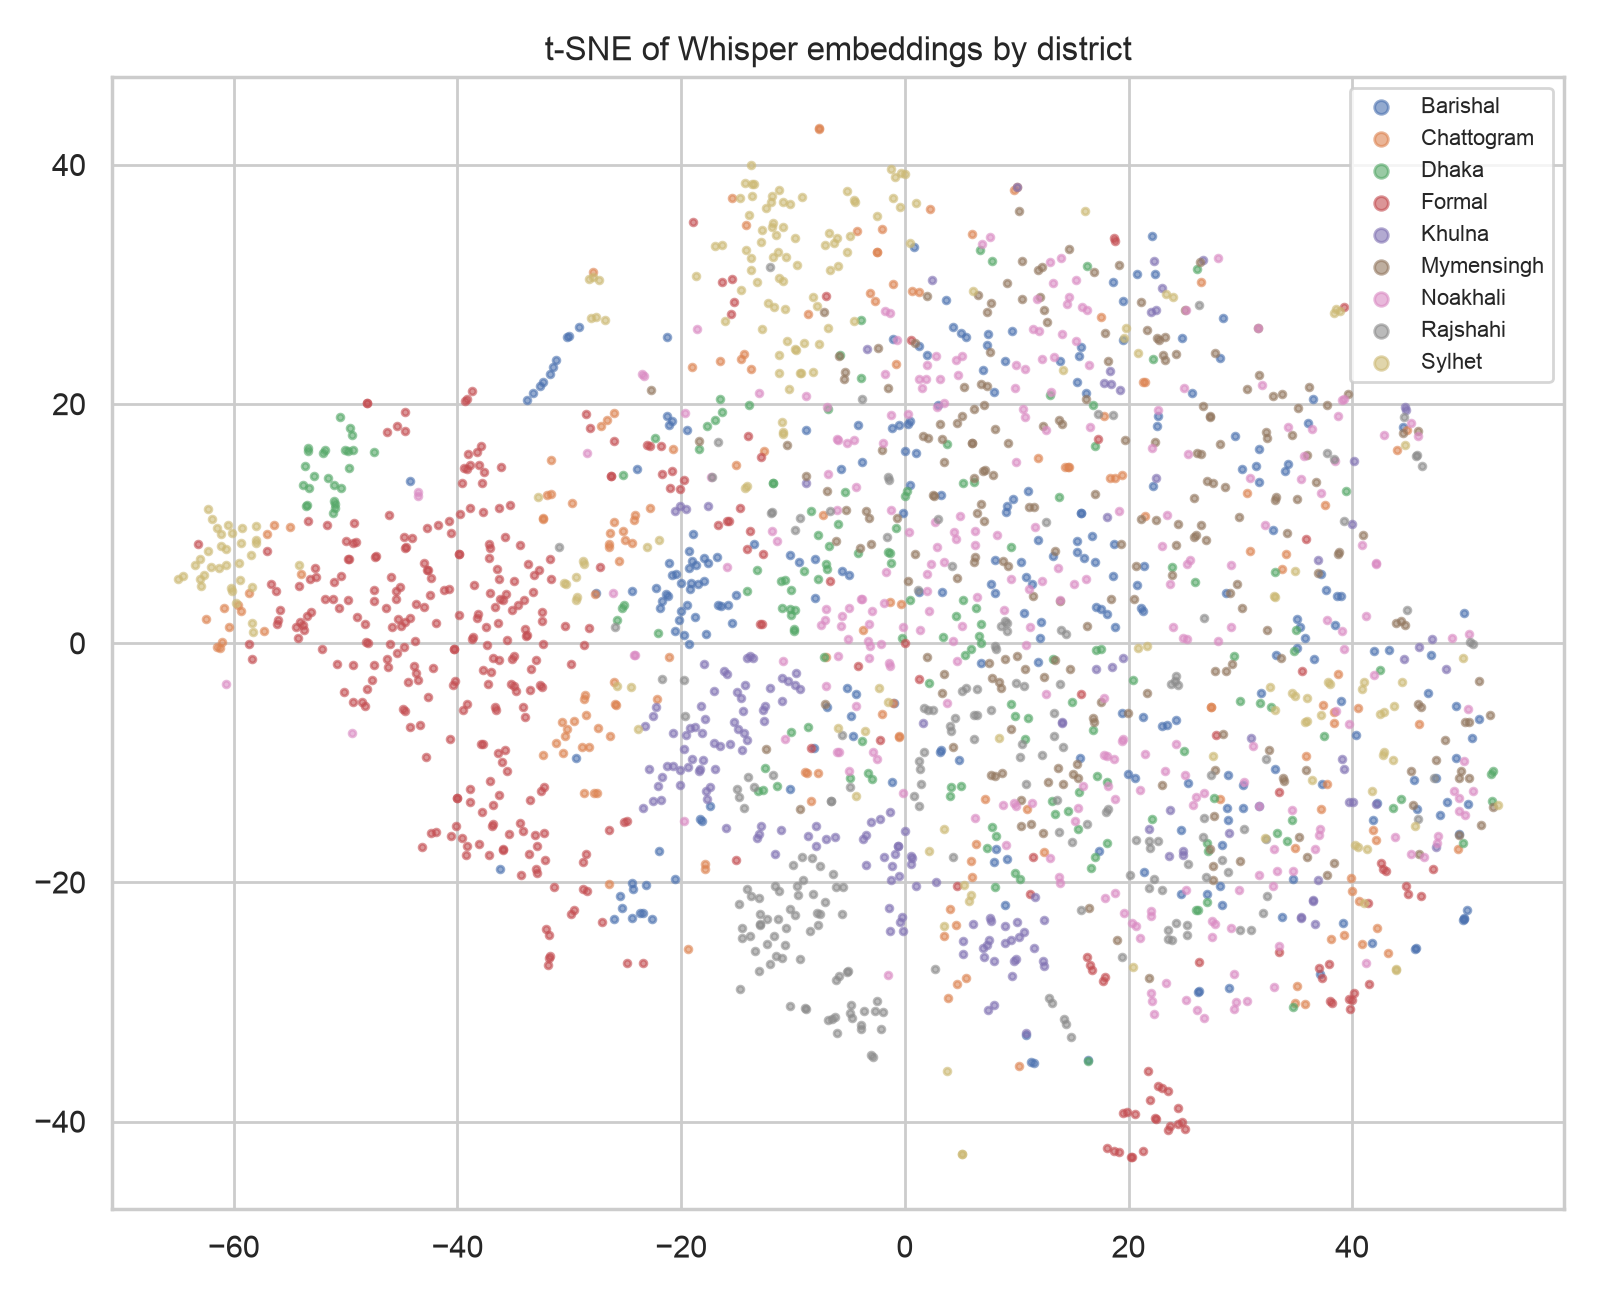
\includegraphics[width=0.7\textwidth]{tsne_embeddings.png}
  \caption{t-SNE projection of frozen Whisper-small embeddings, coloured by
  class.}
  \label{fig:tsne}
\end{figure}

\section{Strict-split results: quantifying leakage}
\label{sec:res-strict}

\Cref{tab:ablation} and \cref{fig:ablation} cross the three representations
with the two split protocols, and add the augmentation variant of
\cref{sec:method-acoustic}.

\begin{table}[ht]
  \centering
  \caption{Representation $\times$ split protocol: test macro-F1.}
  \label{tab:ablation}
  \begin{tabular}{lccc}
    \toprule
    Representation & Clip-level & Strict & $\Delta$ (points) \\
    \midrule
    MFCC statistics + MLP          & 0.727 & 0.480 & $-24.8$ \\
    Frozen Whisper-small + MLP     & 0.917 & 0.793 & $-12.4$ \\
    Fine-tuned XLS-R-300M          & 0.952 & 0.808 & $-14.4$ \\
    XLS-R-300M + channel augmentation & --- & 0.748 & --- \\
    \bottomrule
  \end{tabular}
\end{table}

\begin{figure}[ht]
  \centering
  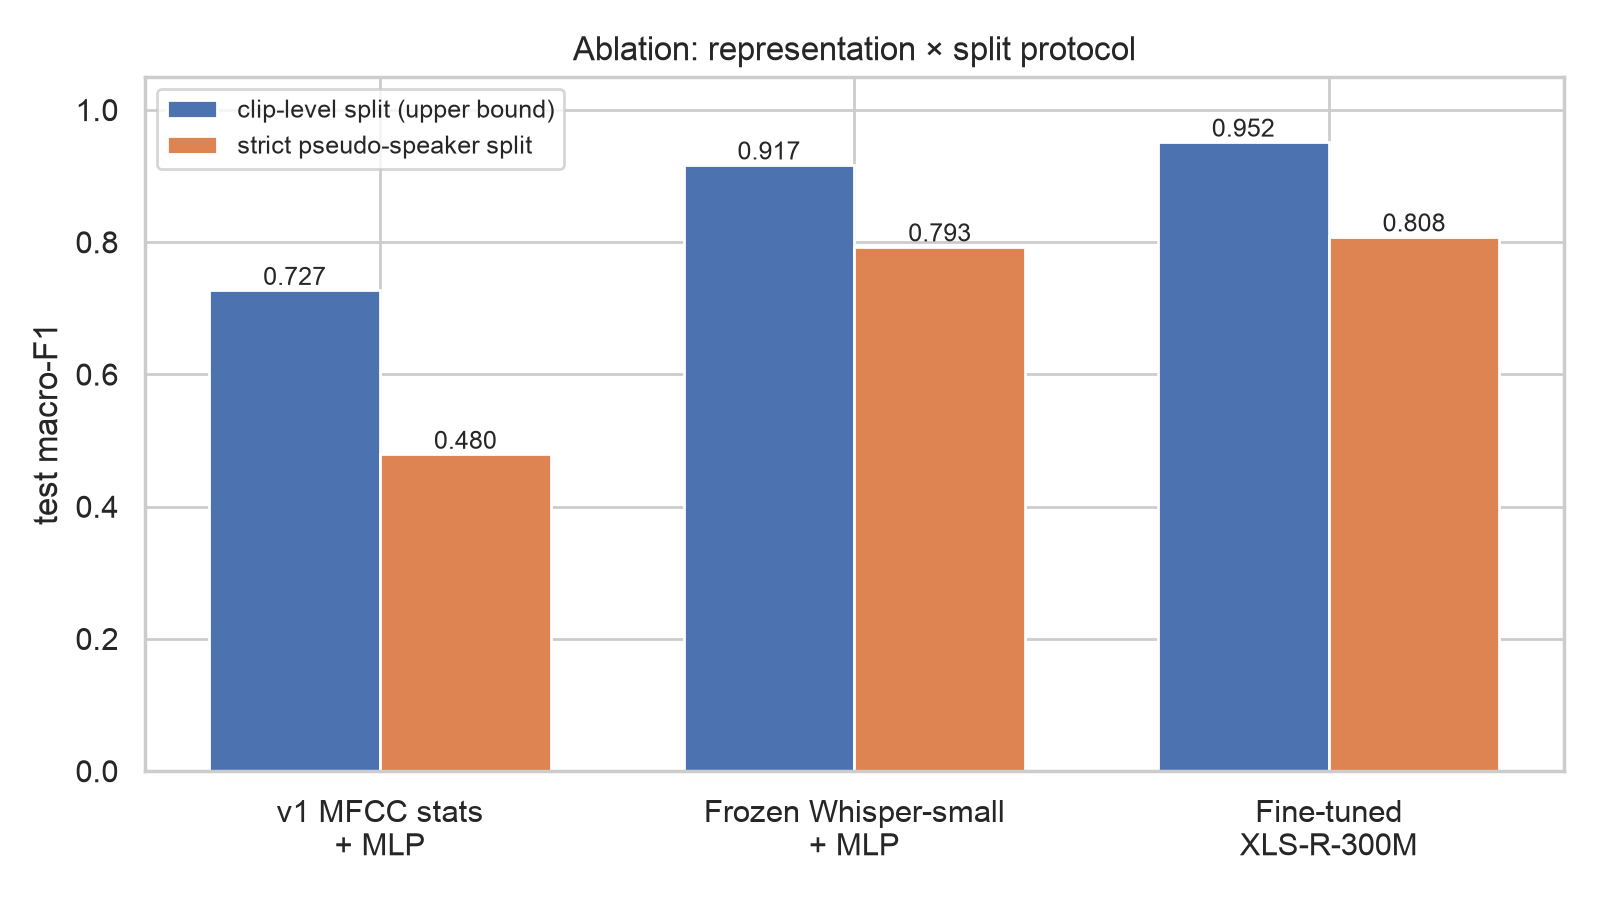
\includegraphics[width=0.85\textwidth]{ablation_representation_split.png}
  \caption{Test macro-F1 for each representation under the clip-level split
  (upper bound) and the strict pseudo-speaker split.}
  \label{fig:ablation}
\end{figure}

\begin{enumerate}
  \item \textbf{Leakage is measured at 12--14 macro-F1 points} for the
        pretrained models, and about 25 for MFCC features. The strict numbers,
        0.793 and 0.808, are the honest estimates; clip-level numbers are kept
        for comparability with prior work.
  \item \textbf{Under the strict split, fine-tuned and frozen models are
        statistically tied.} XLS-R's 1.5-point lead over frozen Whisper has a
        speaker-group bootstrap 95\,\% confidence interval of $-2.0$ to $+7.5$,
        whereas its 3.5-point clip-level lead ($+1.8$ to $+5.3$) is significant.
        Fine-tuning's strict-split drop ($-14.4$) is slightly larger than the
        frozen model's ($-12.4$).
  \item \textbf{Per-class strict scores are noisier than the macro average}
        (\cref{tab:strict-perclass}). Some strict test cells are dominated by a
        single large pseudo-speaker cluster: Barishal's strict test set is
        essentially one 251-clip cluster, so its strict F1 of 0.603 (Whisper)
        and 0.508 (XLS-R) measures generalisation to one speaker or source more
        than to the class.
\end{enumerate}

\begin{table}[ht]
  \centering
  \caption{Per-class test F1, strict split. Test sizes per class are in
  \cref{tab:classes}.}
  \label{tab:strict-perclass}
  \begin{tabular}{lccc}
    \toprule
    Class & MFCC + MLP & Frozen Whisper + MLP & Fine-tuned XLS-R \\
    \midrule
    Barishal   & 0.130 & 0.603 & 0.508 \\
    Chattogram & 0.456 & 0.670 & 0.820 \\
    Dhaka      & 0.426 & 0.881 & 0.848 \\
    Formal     & 0.694 & 0.929 & 0.785 \\
    Khulna     & 0.679 & 0.887 & 0.957 \\
    Mymensingh & 0.495 & 0.813 & 0.904 \\
    Noakhali   & 0.454 & 0.694 & 0.862 \\
    Rajshahi   & 0.372 & 0.900 & 0.842 \\
    Sylhet     & 0.611 & 0.763 & 0.750 \\
    \midrule
    Macro      & \textbf{0.480} & \textbf{0.793} & \textbf{0.808} \\
    \bottomrule
  \end{tabular}
\end{table}

The two pretrained models fail differently under the strict split: frozen
Whisper is better on Formal, Dhaka and Rajshahi, fine-tuned XLS-R on
Chattogram, Noakhali, Mymensingh and Khulna. Their macro averages are close,
but they are not the same model with different accuracy.

\paragraph{Statistical uncertainty.} \Cref{tab:ci-acoustic} gives the 95\,\%
intervals from the group bootstrap of \cref{sec:method-eval}. Clip bootstrap
intervals are narrower but understate the variance. Under the group bootstrap,
every MFCC-versus-pretrained gap is significant, as are XLS-R's clip-level lead
over Whisper and the augmentation drop ($-6.0$, interval $-9.4$ to $-0.9$);
XLS-R's strict-split lead over Whisper is not.

\begin{table}[ht]
  \centering
  \caption{Test macro-F1 with 95\,\% speaker-group bootstrap intervals
  ($B = 2{,}000$; 565 groups in the clip-level test set, 230 in the strict).}
  \label{tab:ci-acoustic}
  \begin{tabular}{lcc}
    \toprule
    Model & Clip-level & Strict \\
    \midrule
    MFCC + MLP             & 0.727 (0.676--0.753) & 0.480 (0.368--0.552) \\
    Frozen Whisper + MLP   & 0.917 (0.894--0.932) & 0.793 (0.688--0.808) \\
    Fine-tuned XLS-R       & 0.952 (0.935--0.963) & 0.808 (0.717--0.838) \\
    XLS-R + augmentation   & ---                  & 0.748 (0.649--0.792) \\
    \bottomrule
  \end{tabular}
\end{table}

\section{Data efficiency}
\label{sec:res-efficiency}

\Cref{tab:efficiency} and \cref{fig:efficiency} show test macro-F1 when the MLP
heads are trained on fractions of the training split (mean of three seeds).

\begin{table}[ht]
  \centering
  \caption{Test macro-F1 against the fraction of training data used (mean of
  three seeds).}
  \label{tab:efficiency}
  \begin{tabular}{lccccc}
    \toprule
    Fraction of training split & 10\,\% & 25\,\% & 50\,\% & 75\,\% & 100\,\% \\
    \midrule
    Whisper, clip-level & 0.788 & 0.854 & 0.902 & 0.908 & 0.913 \\
    Whisper, strict     & 0.671 & 0.751 & 0.784 & 0.790 & 0.793 \\
    MFCC, clip-level    & 0.522 & 0.618 & 0.675 & 0.707 & 0.726 \\
    MFCC, strict        & 0.371 & 0.434 & 0.475 & 0.489 & 0.494 \\
    \bottomrule
  \end{tabular}
\end{table}

\begin{figure}[ht]
  \centering
  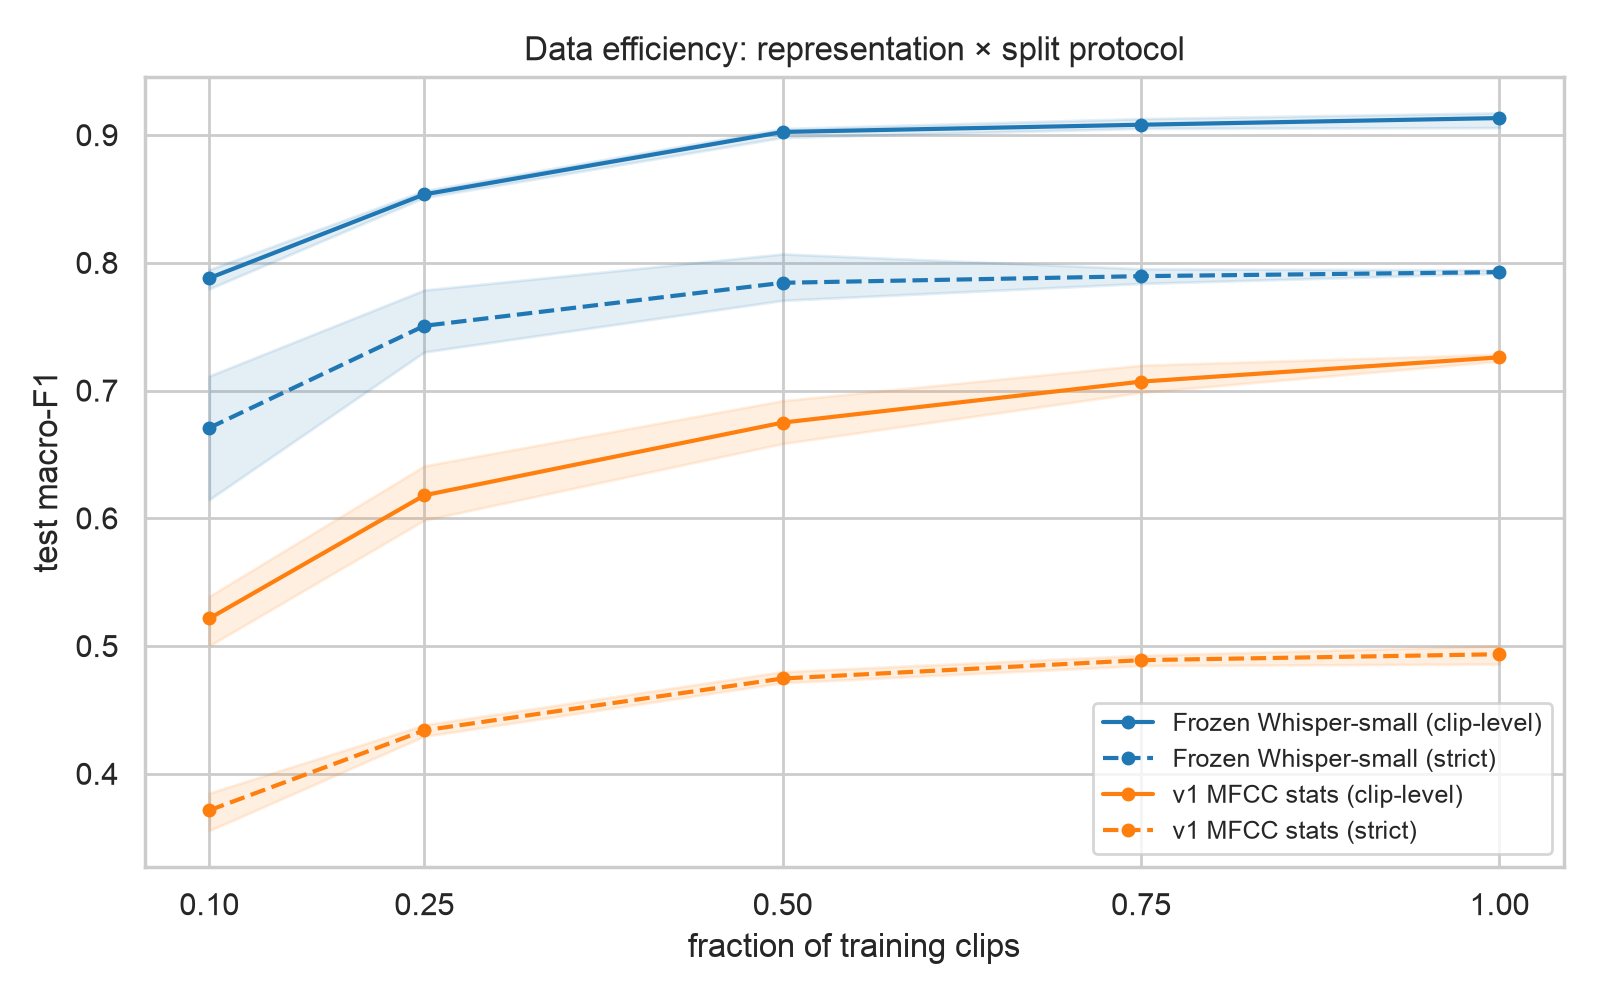
\includegraphics[width=0.85\textwidth]{data_efficiency.png}
  \caption{Data efficiency: test macro-F1 against the fraction of training clips,
  for frozen Whisper and MFCC features under both split protocols. Bands show the
  range over three seeds.}
  \label{fig:efficiency}
\end{figure}

\begin{enumerate}
  \item \textbf{Whisper embeddings trained on 10\,\% of the labels outperform MFCC
        features trained on all of them}, under both protocols. Pretraining is
        worth more than a tenfold increase in labelled data on this task.
  \item The Whisper curves flatten beyond about 50\,\%: the 13-hour corpus is
        adequately sized for the frozen-embedding approach.
  \item The gap between representations is wider under the strict split at every
        fraction, so the pretrained features' robustness to leakage holds across
        data scales.
\end{enumerate}

\section{Augmentation study}
\label{sec:res-augment}

Training the strict-split XLS-R model with the channel-suppression chain of
\cref{sec:method-acoustic} \emph{reduced} test macro-F1 from 0.808 to 0.748. The
validation score was depressed throughout training (best epoch 17 of 20,
validation 0.702 against 0.757 without augmentation), so the drop is not an
artefact of checkpoint selection. \Cref{sec:disc-augment} interprets it.

\section{The lexical route: words versus sound}
\label{sec:res-lexical}

\subsection{How much dialect survives transcription?}
\label{sec:res-asr}

\Cref{tab:asr-quality} scores the five front-ends against the human transcripts
of Ben-10's validation set, which contain 21,119 reference tokens outside the
standard vocabulary.

\begin{table}[ht]
  \centering
  \caption{Speech-recognition quality on Ben-10 validation (1,666 clips, ten
  districts; greedy decoding, punctuation ignored).}
  \label{tab:asr-quality}
  \begin{tabular}{lcccc}
    \toprule
    Front-end & WER & CER & Dialect-word recall & Formal-word recall \\
    \midrule
    Tugstugi (Ben-10)      & \textbf{0.707} & \textbf{0.471} & \textbf{0.192} & \textbf{0.455} \\
    Tugstugi               & 0.775 & 0.532 & 0.034 & 0.369 \\
    Hishab FastConformer   & 0.792 & 0.517 & 0.012 & 0.405 \\
    wav2vec2 Bengali       & 0.942 & 0.669 & 0.012 & 0.085 \\
    Whisper-large-v3       & 0.960 & 0.808 & 0.016 & 0.061 \\
    \bottomrule
  \end{tabular}
\end{table}

The ordering and size of the error rates match the Ben-10 benchmark
\citep{dipto2025ben10}, which reports 0.70 for the Ben-10-fine-tuned model on
its private test set and 0.81, 0.87 and 1.13 for Tugstugi, Hishab and
Whisper-large-v3. Even the best front-end reproduces fewer than one dialect word
in five; by district its recall ranges from 0.243 (Sylhet) to 0.135 (Rangpur).
The standard-Bangla models reproduce 1--3\,\% of dialect words. The benchmark's
hand-counted recall for the two Tugstugi models (0.16--0.53 against
0.01--0.09) is thus confirmed at full scale with an automated measure.

On the thesis corpus, which has no references, the same pattern appears in the
share of transcript words outside the standard vocabulary
(\cref{fig:asr-dialect}b). Only the Ben-10 model separates regional clips (25\,\%
on average) from Formal clips (8\,\%) by a wide margin, with recognisable dialect
forms such as \bn{mui}{মুই}, \bn{ai}{আঁই}, \bn{ar}{আঁর}, \bn{hamar}{হামার}, \bn{kita}{কিতা} and \bn{teha}{টেহা}.
Hishab and the base Tugstugi model output almost as few non-standard words on
regional clips (9\,\% and 13\,\%) as on Formal ones (4\,\% and 5\,\%). The
wav2vec~2.0 and Whisper-large-v3 front-ends have high shares for the wrong
reason: misrecognition, and for Whisper-large-v3 repetition loops in 12.3\,\% of
transcripts (one word repeated five or more times in a row) and 2.5--4.8\,\%
empty outputs per class.

\begin{figure}[ht]
  \centering
  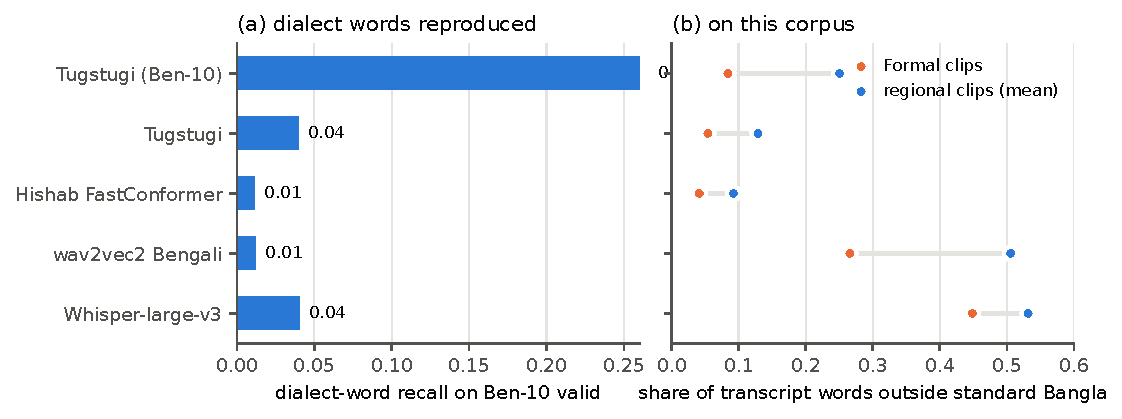
\includegraphics[width=\textwidth]{phase5_asr_dialect.pdf}
  \caption{What survives transcription. (a) Dialect-word recall of each
  front-end on Ben-10 validation. (b) Share of transcript words outside the
  standard vocabulary on this corpus, for Formal clips and the mean over the eight
  regional classes.}
  \label{fig:asr-dialect}
\end{figure}

\subsection{Classification from transcripts}

\Cref{tab:lexical} and \cref{fig:lexical} report the three classifiers for each
front-end, using the in-domain lexicon.

\begin{table}[ht]
  \centering
  \caption{Test macro-F1 of the lexical classifiers by front-end. Fine-tuned
  XLS-R alone scores 0.808 (strict) and 0.952 (clip-level).}
  \label{tab:lexical}
  \small
  \begin{tabular}{lccccc}
    \toprule
    & \multicolumn{3}{c}{Strict} & \multicolumn{2}{c}{Clip-level} \\
    \cmidrule(lr){2-4}\cmidrule(lr){5-6}
    Front-end & Word match & TF-IDF & Fusion & TF-IDF & Fusion \\
    \midrule
    Tugstugi (Ben-10)    & 0.360 & \textbf{0.633} & \textbf{0.856} & \textbf{0.728} & \textbf{0.967} \\
    Tugstugi             & 0.060 & 0.456 & 0.836 & 0.595 & 0.965 \\
    Hishab FastConformer & 0.049 & 0.445 & 0.820 & 0.553 & 0.962 \\
    wav2vec2 Bengali     & 0.077 & 0.424 & 0.825 & 0.536 & 0.960 \\
    Whisper-large-v3     & 0.156 & 0.388 & 0.800 & 0.490 & 0.954 \\
    \bottomrule
  \end{tabular}
\end{table}

\begin{figure}[ht]
  \centering
  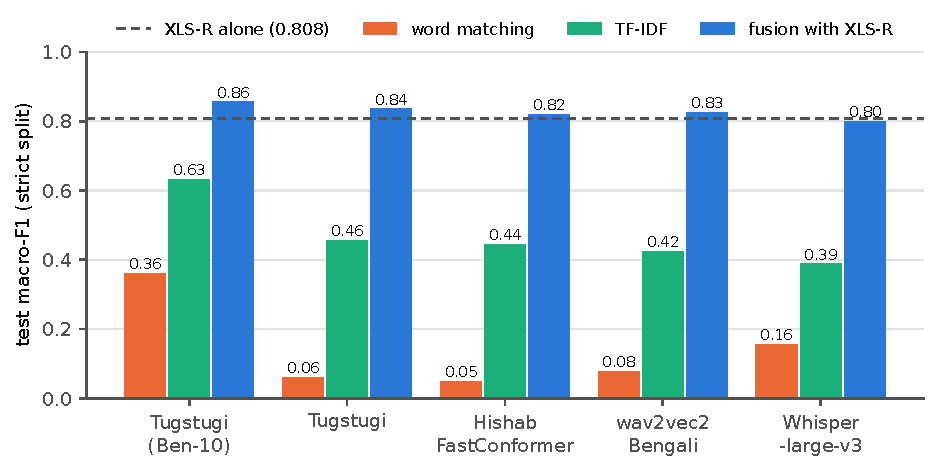
\includegraphics[width=\textwidth]{phase5_classification.pdf}
  \caption{Strict-split test macro-F1 of word matching, the TF-IDF classifier and
  fusion with XLS-R, by speech-recognition front-end. The dashed line is XLS-R
  alone.}
  \label{fig:lexical}
\end{figure}

\begin{enumerate}
  \item \textbf{Word matching is weak} even with the best front-end: 0.360
        strict and 0.399 clip-level. Fewer than half of the strict test clips
        (44\,\%) contain any lexicon word, so the rest default to Formal.
        Relaxing the lexicon thresholds raises coverage to 59\,\% and macro-F1
        to 0.419, still far below every pretrained acoustic model. The clean
        external lexicon (Ben-10 and Vashantor; six classes including Formal)
        scores 0.418 on its own classes with 51\,\% coverage. With the
        standard-Bangla front-ends, coverage collapses to 2--5\,\% and matching
        fails: there are no regional words left to match.
  \item \textbf{The TF-IDF classifier roughly doubles the matching score}
        (0.633 strict with the Ben-10 model), placing the words alone between
        MFCC features (0.480) and frozen Whisper (0.793). The front-ends rank
        exactly as their word error rates on Ben-10 do
        (\cref{tab:asr-quality}).
  \item \textbf{Fusion improves on XLS-R with four of the five front-ends.} With
        the Ben-10 model the strict score rises from 0.808 to 0.856
        ($\alpha = 0.25$, so after tuning the text carries three quarters of the
        log-probability weight) and the clip-level score from 0.952 to 0.967
        ($\alpha = 0.30$).
\end{enumerate}

\subsection{Statistical uncertainty}

\Cref{tab:ci-lexical} gives intervals for the Ben-10 front-end, and
\cref{tab:fusion-gains} the fusion gain over XLS-R for every front-end.

\begin{table}[ht]
  \centering
  \caption{Lexical-route test macro-F1 with 95\,\% speaker-group bootstrap
  intervals (Ben-10 front-end).}
  \label{tab:ci-lexical}
  \begin{tabular}{lcc}
    \toprule
    Model & Clip-level & Strict \\
    \midrule
    Word matching          & 0.399 (0.359--0.421) & 0.360 (0.284--0.380) \\
    TF-IDF                 & 0.728 (0.684--0.748) & 0.633 (0.538--0.642) \\
    Fusion XLS-R + TF-IDF  & 0.967 (0.952--0.976) & 0.856 (0.754--0.875) \\
    Fine-tuned XLS-R (reference) & 0.952 (0.935--0.963) & 0.808 (0.717--0.838) \\
    \bottomrule
  \end{tabular}
\end{table}

\begin{table}[ht]
  \centering
  \caption{Fusion gain over XLS-R alone in macro-F1 points, with 95\,\%
  speaker-group bootstrap interval and the bootstrap probability of no gain.}
  \label{tab:fusion-gains}
  \small
  \begin{tabular}{lcccc}
    \toprule
    & \multicolumn{2}{c}{Clip-level} & \multicolumn{2}{c}{Strict} \\
    \cmidrule(lr){2-3}\cmidrule(lr){4-5}
    Front-end & Gain (CI) & $P(\le 0)$ & Gain (CI) & $P(\le 0)$ \\
    \midrule
    Tugstugi (Ben-10)    & $+1.5$ ($+0.9$, $+2.4$) & 0.000 & $+4.8$ ($-0.3$, $+6.8$) & 0.04 \\
    Tugstugi             & $+1.3$ ($+0.5$, $+2.2$) & 0.002 & $+2.7$ ($-1.0$, $+4.2$) & 0.20 \\
    Hishab FastConformer & $+1.0$ ($+0.4$, $+1.7$) & 0.001 & $+1.1$ ($-2.0$, $+2.2$) & 0.39 \\
    wav2vec2 Bengali     & $+0.8$ ($+0.1$, $+1.7$) & 0.015 & $+1.7$ ($-0.2$, $+3.1$) & 0.04 \\
    Whisper-large-v3     & $+0.2$ ($-0.7$, $+1.1$) & 0.32  & $-0.8$ ($-3.8$, $+0.6$) & 0.90 \\
    \bottomrule
  \end{tabular}
\end{table}

At clip level the fusion gain is significant for every front-end except
Whisper-large-v3. Under the strict split no interval excludes zero; the Ben-10
and wav2vec~2.0 front-ends come closest (a 4\,\% bootstrap probability of no
gain), and with Whisper-large-v3 fusion is slightly worse than XLS-R alone.

\subsection{Where the words help}

\Cref{tab:fusion-perclass} and \cref{fig:fusion-perclass} break the strict-split
result down by class for the Ben-10 front-end.

\begin{table}[ht]
  \centering
  \caption{Per-class test F1, strict split, Ben-10 front-end.}
  \label{tab:fusion-perclass}
  \begin{tabular}{lccccc}
    \toprule
    Class & Word match & TF-IDF & XLS-R & Fusion & $\Delta$ fusion $-$ XLS-R \\
    \midrule
    Barishal   & 0.268 & 0.544 & 0.508 & 0.720 & $\mathbf{+21.2}$ \\
    Sylhet     & 0.600 & 0.750 & 0.750 & 0.832 & $+8.2$ \\
    Chattogram & 0.392 & 0.617 & 0.820 & 0.878 & $+5.8$ \\
    Formal     & 0.448 & 0.805 & 0.785 & 0.835 & $+5.0$ \\
    Noakhali   & 0.500 & 0.707 & 0.862 & 0.898 & $+3.5$ \\
    Mymensingh & 0.395 & 0.694 & 0.904 & 0.928 & $+2.4$ \\
    Rajshahi   & 0.175 & 0.550 & 0.842 & 0.857 & $+1.5$ \\
    Dhaka      & 0.158 & 0.470 & 0.848 & 0.853 & $+0.5$ \\
    Khulna     & 0.305 & 0.557 & 0.957 & 0.904 & $-5.3$ \\
    \bottomrule
  \end{tabular}
\end{table}

\begin{figure}[ht]
  \centering
  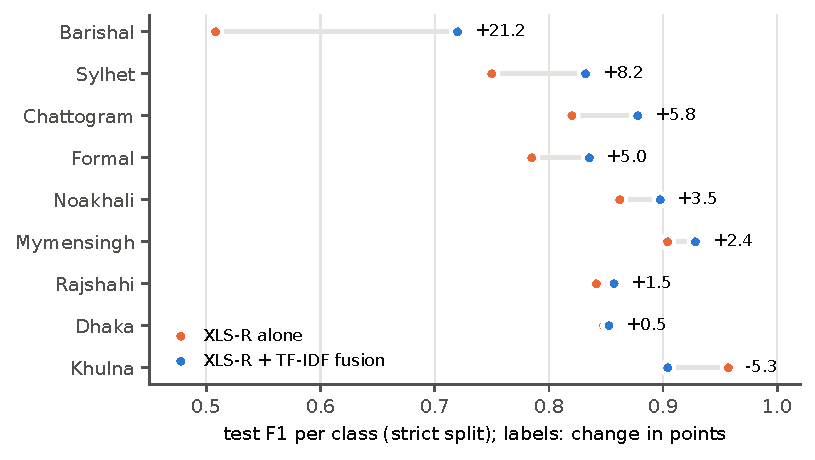
\includegraphics[width=0.8\textwidth]{phase5_fusion_per_class.pdf}
  \caption{Per-class test F1 on the strict split for XLS-R alone and for its
  fusion with the TF-IDF transcript classifier (Ben-10 front-end). Labels give
  the change in F1 points.}
  \label{fig:fusion-perclass}
\end{figure}

The gain concentrates on the classes the acoustic model finds hardest under the
strict split---Barishal, the single-cluster test cell, and Sylhet---and on the
classes with the most distinctive, best-transcribed vocabulary: Sylhet's match
F1 of 0.600 is the only strong word-matching result. Khulna, the acoustic
model's best class, is the one class that fusion hurts. Formal is the only class
on which the text classifier alone beats XLS-R: the standard register is marked
in its vocabulary.
